%!TeX root=../wowtop.tex

\ArtChapter[In London]{14head}



\lettrine[lines=4,findent=2pt]{M}{y} younger brother was in London when the Martians fell at Woking. He was a medical student working for an imminent examination, and he heard nothing of the arrival until Saturday morning. The morning papers on Saturday contained, in addition to lengthy special articles on the planet Mars, on life in the planets, and so forth, a brief and vaguely worded telegram, all the more striking for its brevity.

The Martians, alarmed by the approach of a crowd, had killed a number of people with a quick-firing gun, so the story ran. The telegram concluded with the words: »Formidable as they seem to be, the Martians have not moved from the pit into which they have fallen, and, indeed, seem incapable of doing so. Probably this is due to the relative strength of the earth's gravitational energy.« On that last text their leader-writer expanded very comfortingly.

Of course all the students in the crammer's biology class, to which my brother went that day, were intensely interested, but there were no signs of any unusual excitement in the streets. The afternoon papers puffed scraps of news under big headlines. They had nothing to tell beyond the movements of troops about the common, and the burning of the pine woods between Woking and Weybridge, until eight. Then the \textit{St~James's Gazette}, in an extra-special edition, announced the bare fact of the interruption of telegraphic communication. This was thought to be due to the falling of burning pine trees across the line. Nothing more of the fighting was known that night, the night of my drive to Leatherhead and back.

My brother felt no anxiety about us, as he knew from the description in the papers that the cylinder was a good two miles from my house. He made up his mind to run down that night to me, in order, as he says, to see the Things before they were killed. He dispatched a telegram, which never reached me, about four o'clock, and spent the evening at a music hall.

\begin{figure}[bh!]
\centering

\includegraphics[width=\textwidth]{14destruction}
\end{figure}

%\begin{wrapfigure}{O}{0.5\textwidth}
%\centering
%
\includegraphics[width=0.5\textwidth]{14destruction}
%\end{wrapfigure}

In London, also, on Saturday night there was a thunderstorm, and my brother reached Waterloo in a cab. On the platform from which the midnight train usually starts he learned, after some waiting, that an accident prevented trains from reaching Woking that night.\label{brojourney1a} The nature of the accident he could not ascertain; indeed, the railway authorities did not clearly know at that time. There was very little excitement in the station, as the officials, failing to realise that anything further than a breakdown between Byfleet and Woking junction had occurred, were running the theatre trains which usually passed through Woking round by Virginia Water or Guildford. They were busy making the necessary arrangements to alter the route of the Southampton and Portsmouth Sunday League excursions. A nocturnal newspaper reporter, mistaking my brother for the traffic manager, to whom he bears a slight resemblance, waylaid and tried to interview him. Few people, excepting the railway officials, connected the breakdown with the Martians.

I have read, in another account of these events, that on Sunday morning »all London was electrified by the news from Woking.« As a matter of fact, there was nothing to justify that very extravagant phrase. Plenty of Londoners did not hear of the Martians until the panic of Monday morning. Those who did took some time to realise all that the hastily worded telegrams in the Sunday papers conveyed. The majority of people in London do not read Sunday papers.

\begin{figure}[th!]
\centering
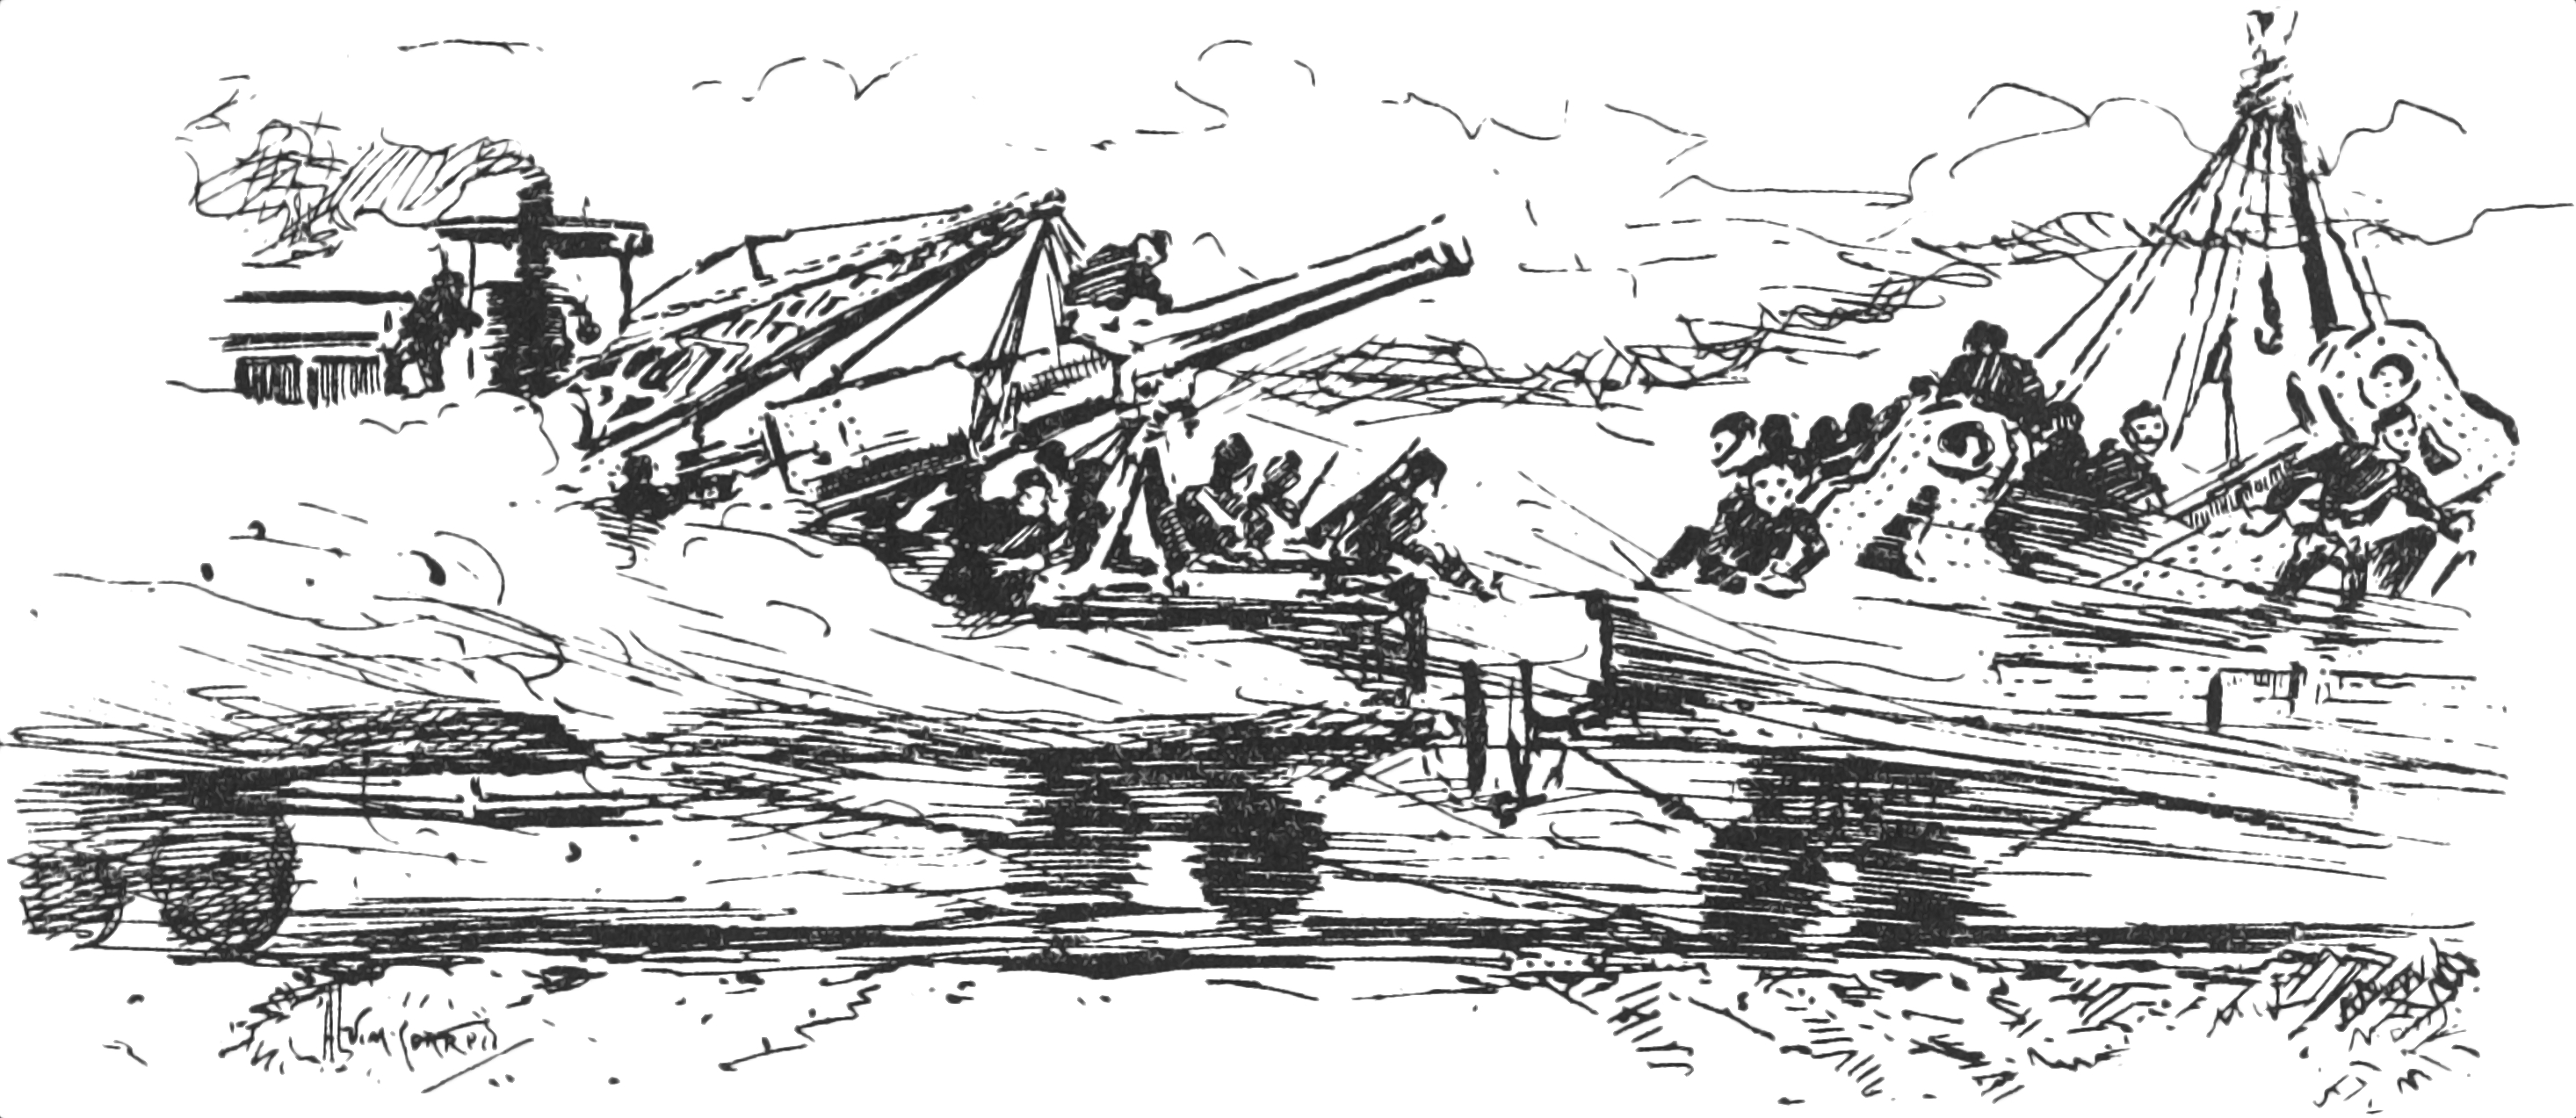
\includegraphics[width=\textwidth]{14boats}
\end{figure}

%\begin{wrapfigure}{O}{0.5\textwidth}
%\centering
%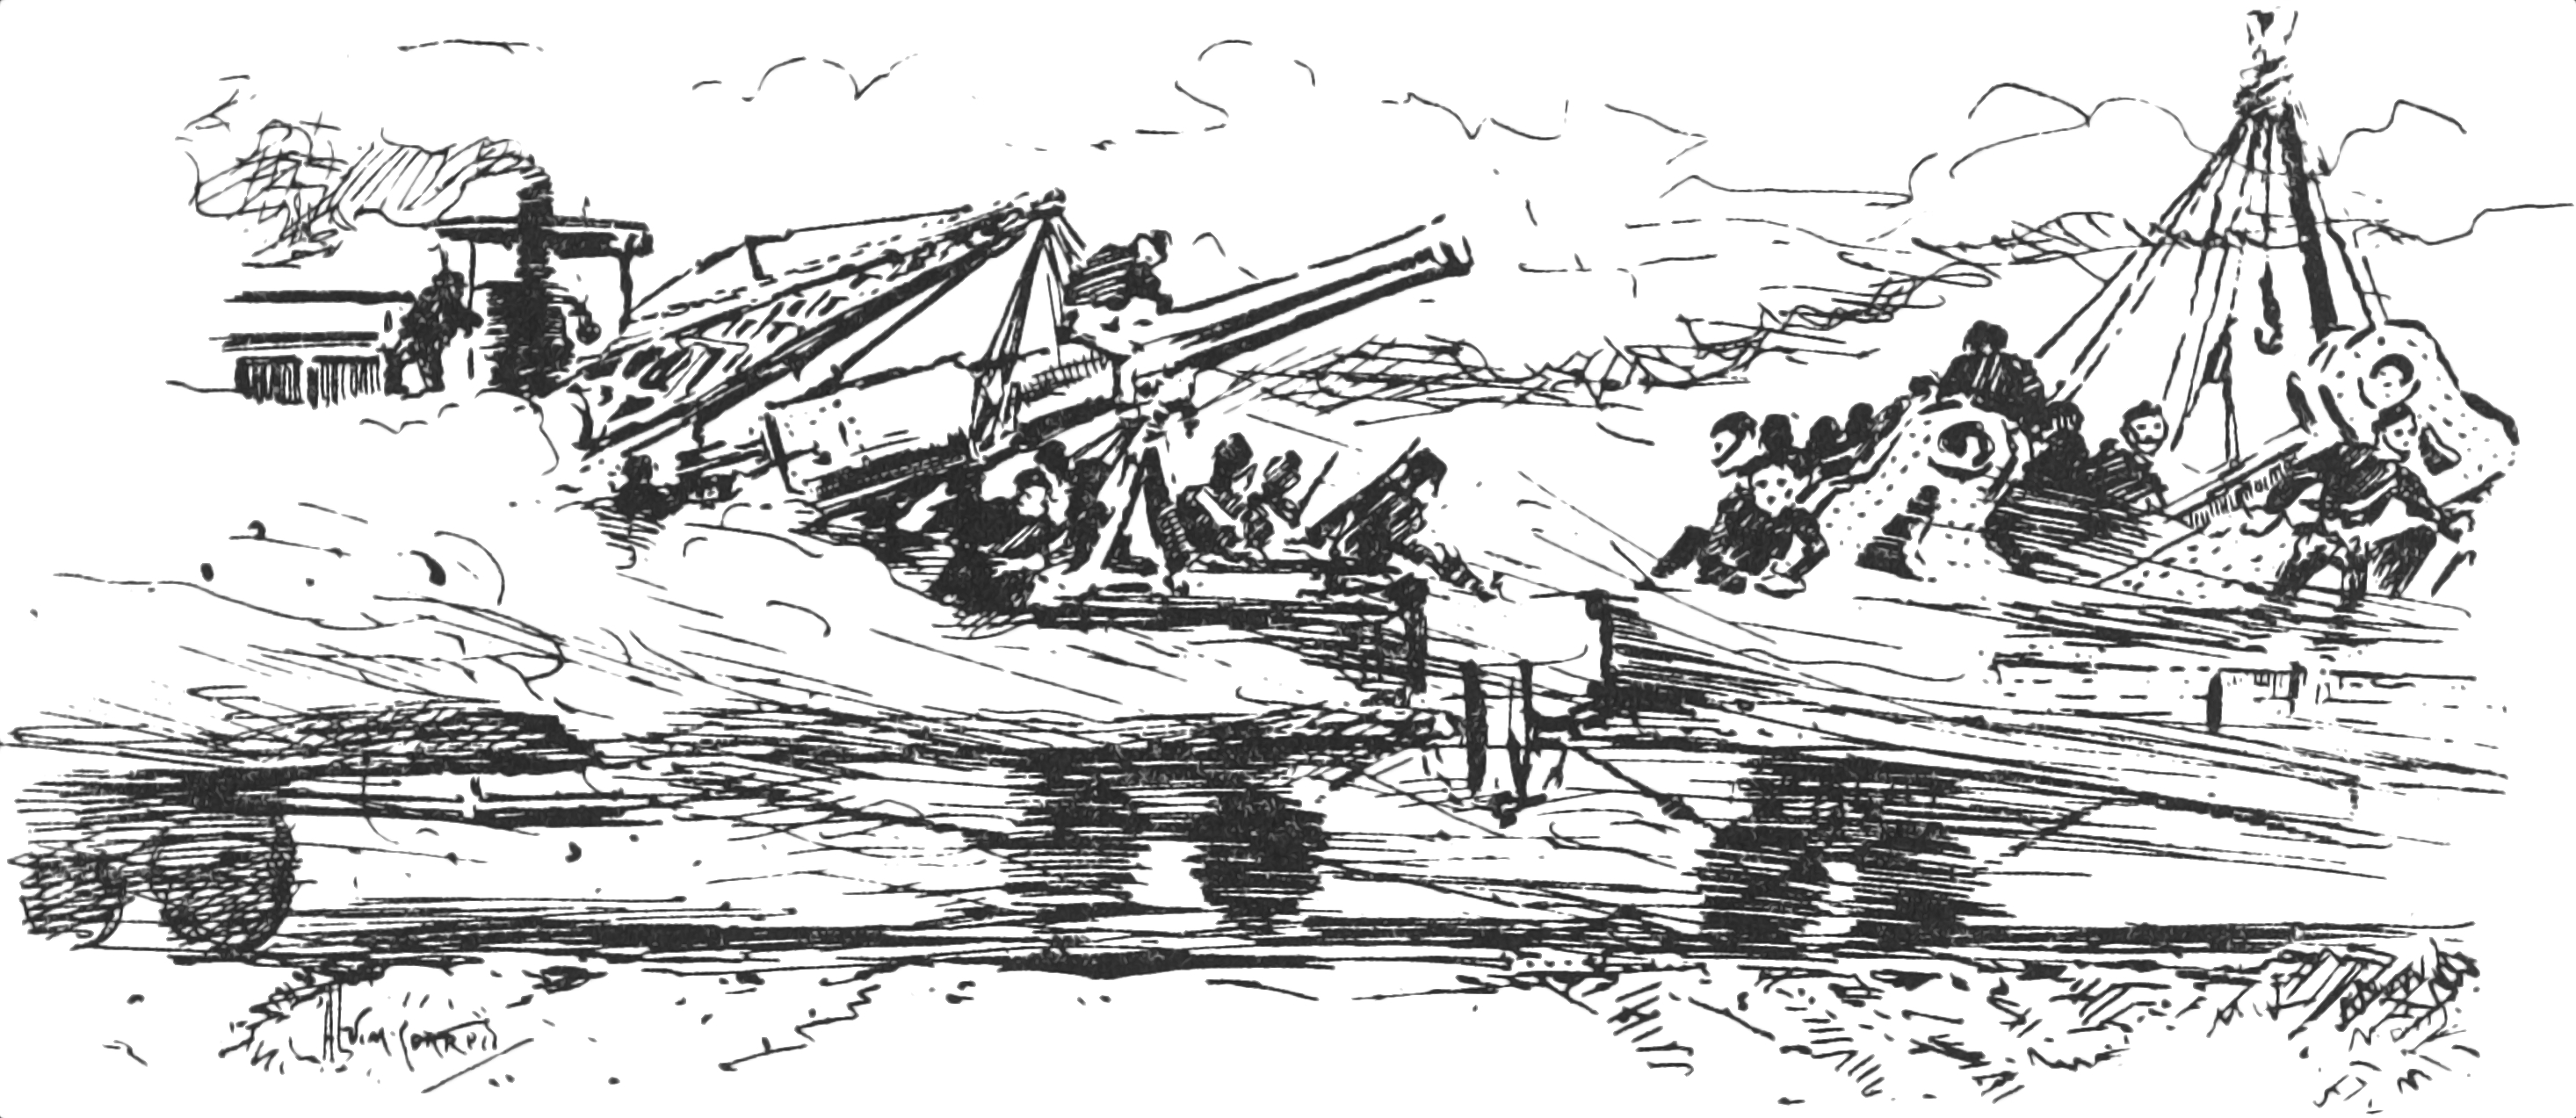
\includegraphics[width=0.5\textwidth]{14boats}
%\end{wrapfigure}

The habit of personal security, moreover, is so deeply fixed in the Londoner's mind, and startling intelligence so much a matter of course in the papers, that they could read without any personal tremors: »About seven o'clock last night the Martians came out of the cylinder, and, moving about under an armour of metallic shields, have completely wrecked Woking station with the adjacent houses, and massacred an entire battalion of the Cardigan Regiment. No details are known. Maxims have been absolutely useless against their armour; the field guns have been disabled by them. Flying hussars have been galloping into Chertsey. The Martians appear to be moving slowly towards Chertsey or Windsor. Great anxiety prevails in West Surrey, and earthworks are being thrown up to check the advance Londonward.« That was how the \textit{Sunday Sun} put it, and a clever and remarkably prompt »handbook« article in the \textit{Referee} compared the affair to a menagerie suddenly let loose in a village.

No one in London knew positively of the nature of the armoured Martians, and there was still a fixed idea that these monsters must be sluggish: »crawling,« »creeping painfully«—such expressions occurred in almost all the earlier reports. None of the telegrams could have been written by an eyewitness of their advance. The Sunday papers printed separate editions as further news came to hand, some even in default of it. But there was practically nothing more to tell people until late in the afternoon, when the authorities gave the press agencies the news in their possession. It was stated that the people of Walton and Weybridge, and all the district were pouring along the roads Londonward, and that was all.

My brother went to church at the Foundling Hospital \label{brojourney2a} in the morning, still in ignorance of what had happened on the previous night. There he heard allusions made to the invasion, and a special prayer for peace. Coming out, he bought a \textit{Referee}. He became alarmed at the news in this, and went again to Waterloo station \label{brojourney1b} to find out if communication were restored. The omnibuses, carriages, cyclists, and innumerable people walking in their best clothes seemed scarcely affected by the strange intelligence that the newsvendors were disseminating. People were interested, or, if alarmed, alarmed only on account of the local residents. At the station he heard for the first time that the Windsor and Chertsey lines were now interrupted. The porters told him that several remarkable telegrams had been received in the morning from Byfleet and Chertsey stations, but that these had abruptly ceased. My brother could get very little precise detail out of them.

»There's fighting going on about Weybridge« was the extent of their information.

The train service was now very much disorganised. Quite a number of people who had been expecting friends from places on the South-Western network were standing about the station. One grey-headed old gentleman came and abused the South-Western Company bitterly to my brother. »It wants showing up,« he said.

One or two trains came in from Richmond, Putney, and Kingston, containing people who had gone out for a day's boating and found the locks closed and a feeling of panic in the air. A man in a blue and white blazer addressed my brother, full of strange tidings.

»There's hosts of people driving into Kingston in traps and carts and things, with boxes of valuables and all that,« he said. »They come from Molesey and Weybridge and Walton, and they say there's been guns heard at Chertsey, heavy firing, and that mounted soldiers have told them to get off at once because the Martians are coming. We heard guns firing at Hampton Court station, but we thought it was thunder. What the dickens does it all mean? The Martians can't get out of their pit, can they?«

My brother could not tell him.

Afterwards he found that the vague feeling of alarm had spread to the clients of the underground railway, and that the Sunday excursionists began to return from all over the South-Western »lung«—Barnes, Wimbledon, Richmond Park, Kew, and so forth—at unnaturally early hours; but not a soul had anything more than vague hearsay to tell of. Everyone connected with the terminus seemed ill-tempered.

About five o'clock the gathering crowd in the station was immensely excited by the opening of the line of communication, which is almost invariably closed, between the South-Eastern and the South-Western stations, and the passage of carriage trucks bearing huge guns and carriages crammed with soldiers. These were the guns that were brought up from Woolwich and Chatham to cover Kingston. There was an exchange of pleasantries: »You'll get eaten!« »We're the beast-tamers!« and so forth. A little while after that a squad of police came into the station and began to clear the public off the platforms, and my brother went out into the street again.

\begin{wrapfigure}{O}{0.5\textwidth}
\centering

\includegraphics[width=0.5\textwidth]{14crowd}
\end{wrapfigure}

The church bells were ringing for evensong, and a squad of Salvation Army lassies came singing down Waterloo Road. On the bridge a number of loafers were watching a curious brown scum that came drifting down the stream in patches. The sun was just setting, and the Clock Tower and the Houses of Parliament rose against one of the most peaceful skies it is possible to imagine, a sky of gold, barred with long transverse stripes of reddish-purple cloud. There was talk of a floating body. One of the men there, a reservist he said he was, told my brother he had seen the heliograph flickering in the west.

In Wellington Street my brother met a couple of sturdy roughs who had just been rushed out of Fleet Street with still-wet newspapers and staring placards. \label{brojourney3} »Dreadful catastrophe!« they bawled one to the other down Wellington Street. »Fighting at Weybridge! Full description! Repulse of the Martians! London in Danger!« He had to give threepence for a copy of that paper.

Then it was, and then only, that he realised something of the full power and terror of these monsters. He learned that they were not merely a handful of small sluggish creatures, but that they were minds swaying vast mechanical bodies; and that they could move swiftly and smite with such power that even the mightiest guns could not stand against them.

They were described as »vast spiderlike machines, nearly a hundred feet high, capable of the speed of an express train, and able to shoot out a beam of intense heat.« Masked batteries, chiefly of field guns, had been planted in the country about Horsell Common, and especially between the Woking district and London. Five of the machines had been seen moving towards the Thames, and one, by a happy chance, had been destroyed. In the other cases the shells had missed, and the batteries had been at once annihilated by the Heat-Rays. Heavy losses of soldiers were mentioned, but the tone of the dispatch was optimistic.

The Martians had been repulsed; they were not invulnerable. They had retreated to their triangle of cylinders again, in the circle about Woking. Signallers with heliographs were pushing forward upon them from all sides. Guns were in rapid transit from Windsor, Portsmouth, Aldershot, Woolwich—even from the north; among others, long wire-guns of ninety-five tons from Woolwich. Altogether one hundred and sixteen were in position or being hastily placed, chiefly covering London. Never before in England had there been such a vast or rapid concentration of military material.

Any further cylinders that fell, it was hoped, could be destroyed at once by high explosives, which were being rapidly manufactured and distributed. No doubt, ran the report, the situation was of the strangest and gravest description, but the public was exhorted to avoid and discourage panic. No doubt the Martians were strange and terrible in the extreme, but at the outside there could not be more than twenty of them against our millions.

The authorities had reason to suppose, from the size of the cylinders, that at the outside there could not be more than five in each cylinder—fifteen altogether. And one at least was disposed of—perhaps more. The public would be fairly warned of the approach of danger, and elaborate measures were being taken for the protection of the people in the threatened southwestern suburbs. And so, with reiterated assurances of the safety of London and the ability of the authorities to cope with the difficulty, this quasi-proclamation closed.

This was printed in enormous type on paper so fresh that it was still wet, and there had been no time to add a word of comment. It was curious, my brother said, to see how ruthlessly the usual contents of the paper had been hacked and taken out to give this place.

All down Wellington Street people could be seen fluttering out the pink sheets and reading, and the Strand was suddenly noisy with the voices of an army of hawkers following these pioneers. Men came scrambling off buses to secure copies. Certainly this news excited people intensely, whatever their previous apathy. The shutters of a map shop in the Strand were being taken down, my brother said, and a man in his Sunday raiment, lemon-yellow gloves even, was visible inside the window hastily fastening maps of Surrey to the glass.

\begin{wrapfigure}{O}{0.5\textwidth}
\centering
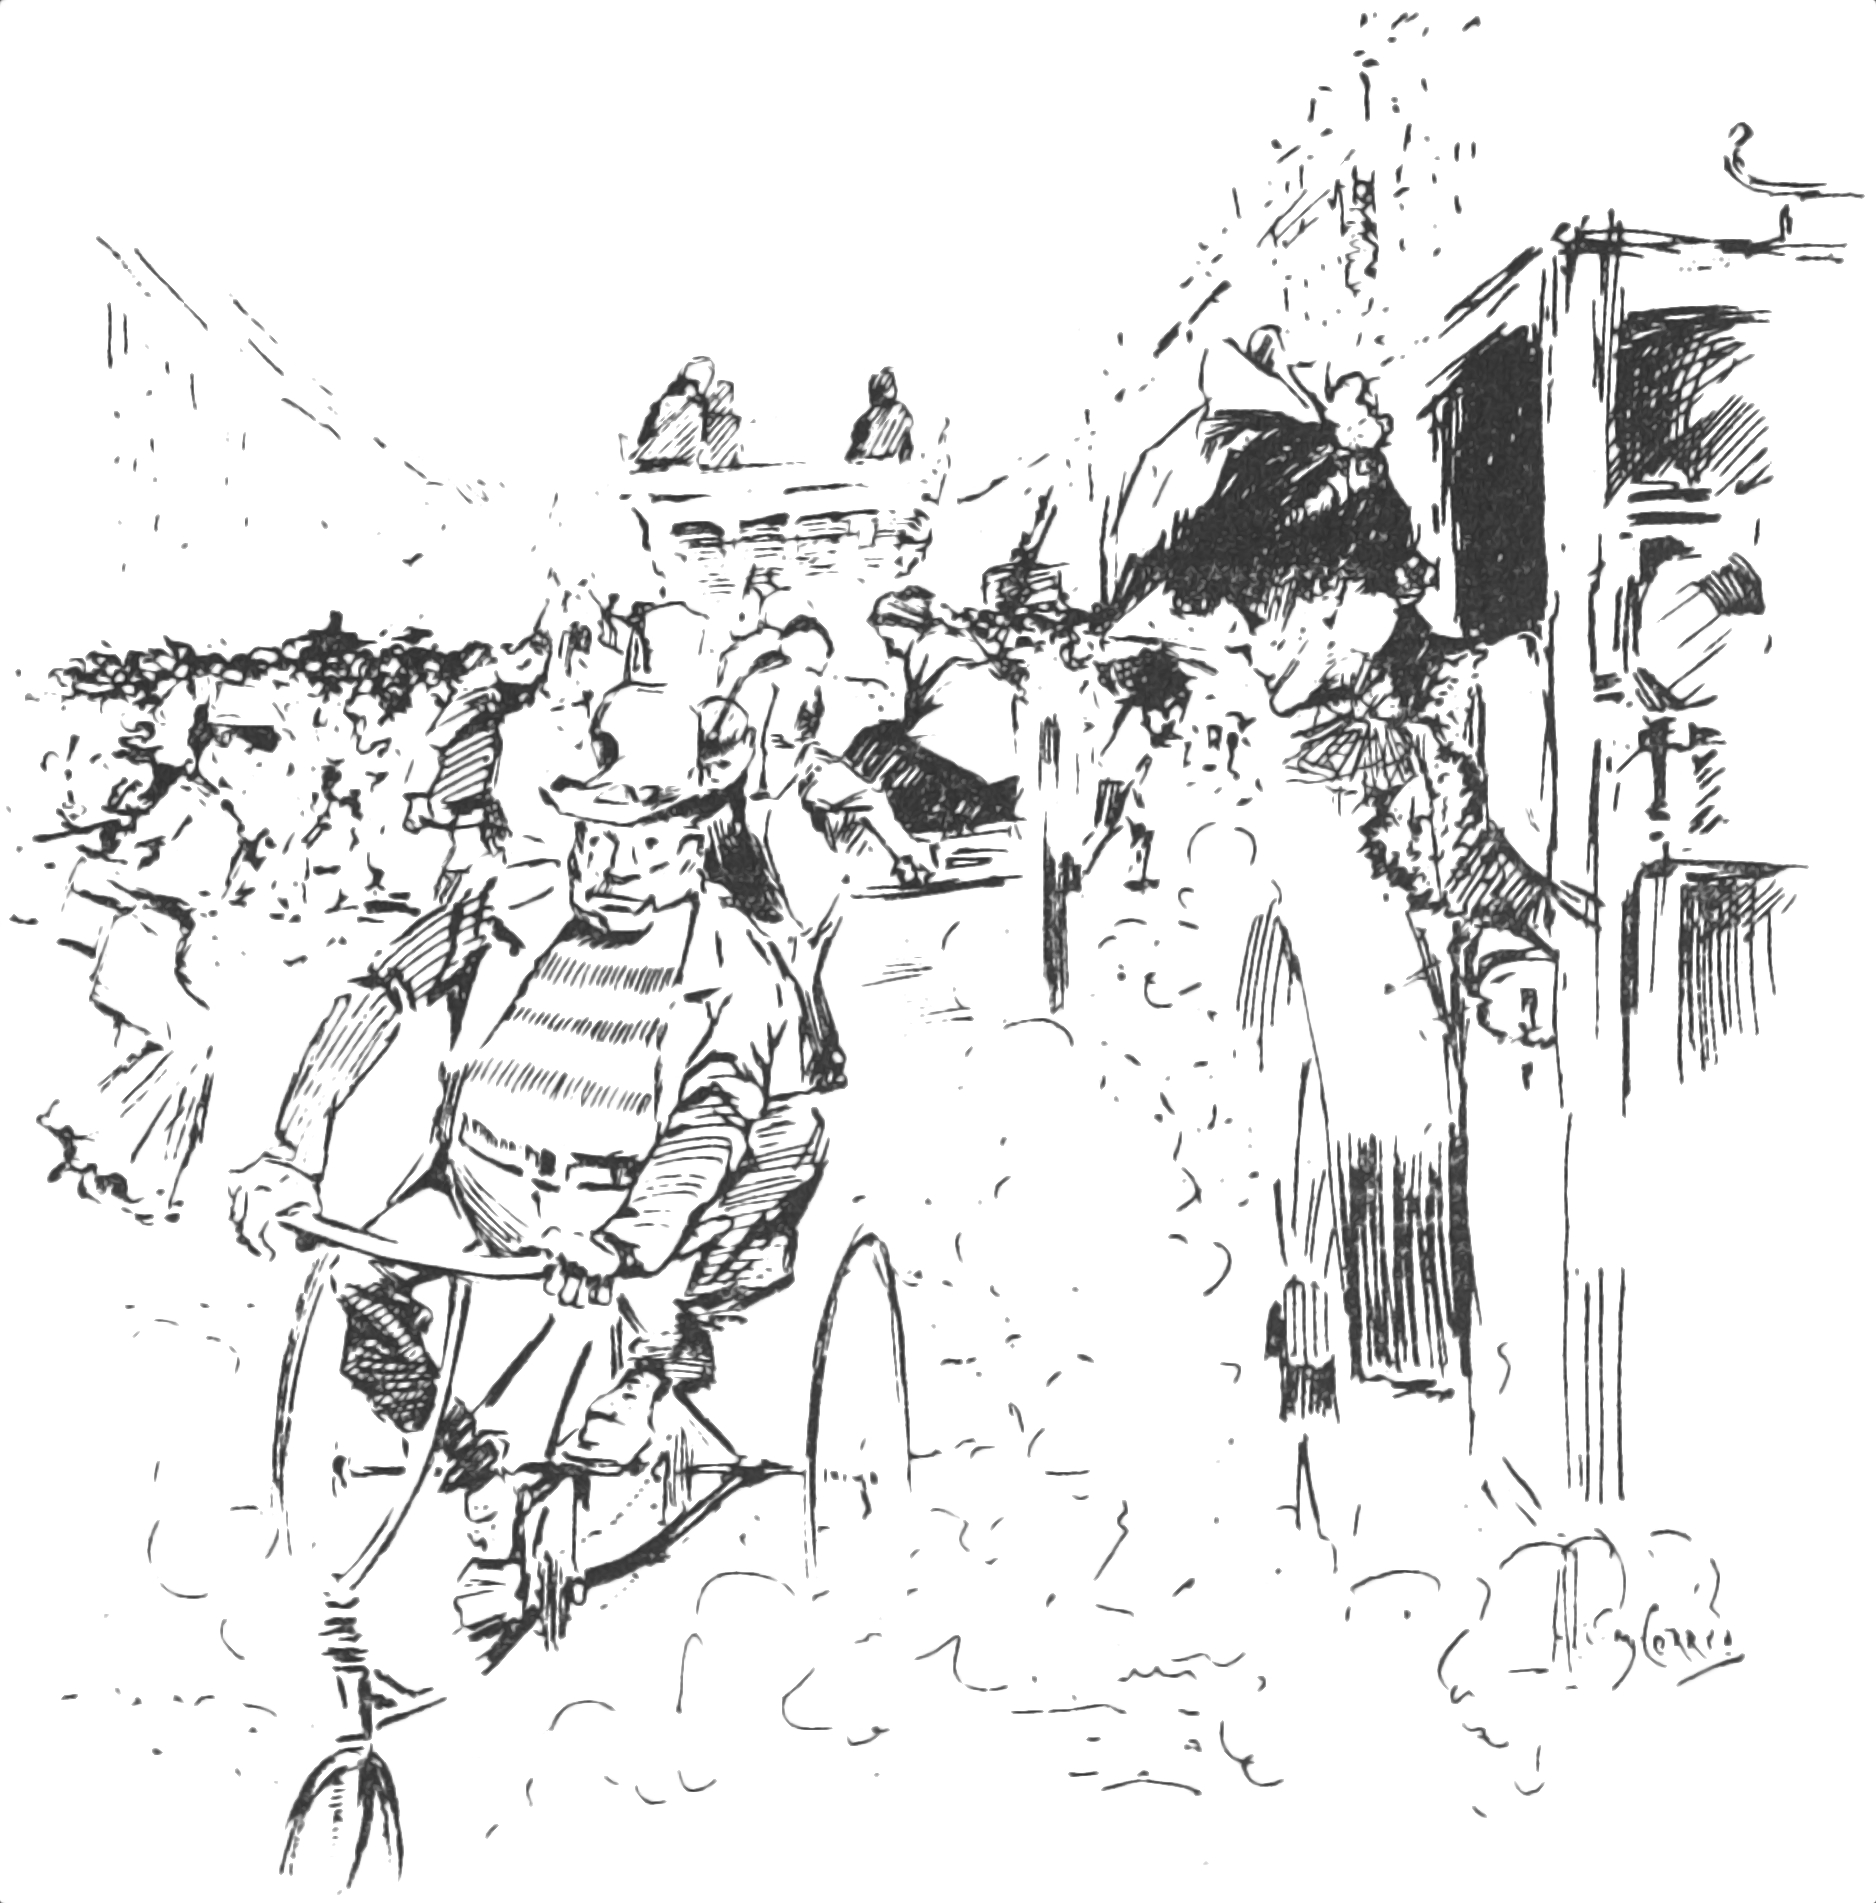
\includegraphics[width=0.5\textwidth]{14trike}
\end{wrapfigure}

Going on along the Strand to Trafalgar Square, the paper in his hand, my brother saw some of the fugitives from West Surrey. \label{brojourney4} There was a man with his wife and two boys and some articles of furniture in a cart such as greengrocers use. He was driving from the direction of Westminster Bridge; and close behind him came a hay waggon with five or six respectable-looking people in it, and some boxes and bundles. The faces of these people were haggard, and their entire appearance contrasted conspicuously with the Sabbath-best appearance of the people on the omnibuses. People in fashionable clothing peeped at them out of cabs. They stopped at the Square as if undecided which way to take, and finally turned eastward along the Strand. Some way behind these came a man in workday clothes, riding one of those old-fashioned tricycles with a small front wheel. He was dirty and white in the face.

My brother turned down towards Victoria,\label{brojourney5} and met a number of such people. He had a vague idea that he might see something of me. He noticed an unusual number of police regulating the traffic. Some of the refugees were exchanging news with the people on the omnibuses. One was professing to have seen the Martians. »Boilers on stilts, I tell you, striding along like men.« Most of them were excited and animated by their strange experience.

Beyond Victoria the public-houses were doing a lively trade with these arrivals. At all the street corners groups of people were reading papers, talking excitedly, or staring at these unusual Sunday visitors. They seemed to increase as night drew on, until at last the roads, my brother said, were like Epsom High Street on a Derby Day. My brother addressed several of these fugitives and got unsatisfactory answers from most.

None of them could tell him any news of Woking except one man, who assured him that Woking had been entirely destroyed on the previous night.

»I come from Byfleet,« he said; »a man on a bicycle came through the place in the early morning, and ran from door to door warning us to come away. Then came soldiers. We went out to look, and there were clouds of smoke to the south—nothing but smoke, and not a soul coming that way. Then we heard the guns at Chertsey, and folks coming from Weybridge. So I've locked up my house and come on.«

At that time there was a strong feeling in the streets that the authorities were to blame for their incapacity to dispose of the invaders without all this inconvenience.

About eight o'clock a noise of heavy firing was distinctly audible all over the south of London. My brother could not hear it for the traffic in the main thoroughfares, but by striking through the quiet back streets to the river he was able to distinguish it quite plainly.

He walked from Westminster to his apartments near Regent's Park,\label{brojourney8} about two. He was now very anxious on my account, and disturbed at the evident magnitude of the trouble. His mind was inclined to run, even as mine had run on Saturday, on military details. He thought of all those silent, expectant guns, of the suddenly nomadic countryside; he tried to imagine »boilers on stilts« a hundred feet high.

\begin{wrapfigure}{O}{0.5\textwidth}
\centering

\includegraphics[width=0.5\textwidth]{14tailpiece}
\end{wrapfigure}

There were one or two cartloads of refugees passing along Oxford Street, and several in the Marylebone Road, but so slowly was the news spreading that Regent Street and Portland Place were full of their usual Sunday-night promenaders, albeit they talked in groups, and along the edge of Regent's Park there were as many silent couples »walking out« together under the scattered gas lamps as ever there had been. The night was warm and still, and a little oppressive; the sound of guns continued intermittently, and after midnight there seemed to be sheet lightning in the south.

He read and re-read the paper, fearing the worst had happened to me. He was restless, and after supper prowled out again aimlessly. He returned and tried in vain to divert his attention to his examination notes. He went to bed a little after midnight, and was awakened from lurid dreams in the small hours of Monday by the sound of door knockers, feet running in the street, distant drumming, and a clamour of bells. Red reflections danced on the ceiling. For a moment he lay astonished, wondering whether day had come or the world gone mad. Then he jumped out of bed and ran to the window.

His room was an attic and as he thrust his head out, up and down the street there were a dozen echoes to the noise of his window sash, and heads in every kind of night disarray appeared. Enquiries were being shouted. »They are coming!« bawled a policeman, hammering at the door; »the Martians are coming!« and hurried to the next door.

The sound of drumming and trumpeting came from the Albany Street Barracks, and every church within earshot was hard at work killing sleep with a vehement disorderly tocsin. There was a noise of doors opening, and window after window in the houses opposite flashed from darkness into yellow illumination.

Up the street came galloping a closed carriage, bursting abruptly into noise at the corner, rising to a clattering climax under the window, and dying away slowly in the distance. Close on the rear of this came a couple of cabs, the forerunners of a long procession of flying vehicles, going for the most part to Chalk Farm station, where the North-Western special trains were loading up, instead of coming down the gradient into Euston.



For a long time my brother stared out of the window in blank astonishment, watching the policemen hammering at door after door, and delivering their incomprehensible message. Then the door behind him opened, and the man who lodged across the landing came in, dressed only in shirt, trousers, and slippers, his braces loose about his waist, his hair disordered from his pillow.

»What the devil is it?« he asked. »A fire? What a devil of a row!«

They both craned their heads out of the window, straining to hear what the policemen were shouting. People were coming out of the side streets, and standing in groups at the corners talking.

»What the devil is it all about?« said my brother's fellow lodger.

My brother answered him vaguely and began to dress, running with each garment to the window in order to miss nothing of the growing excitement. And presently men selling unnaturally early newspapers came bawling into the street:

»London in danger of suffocation! The Kingston and Richmond defences forced! Fearful massacres in the Thames Valley!«

%\begin{wrapfigure}{O}{0.5\textwidth}
%\centering
%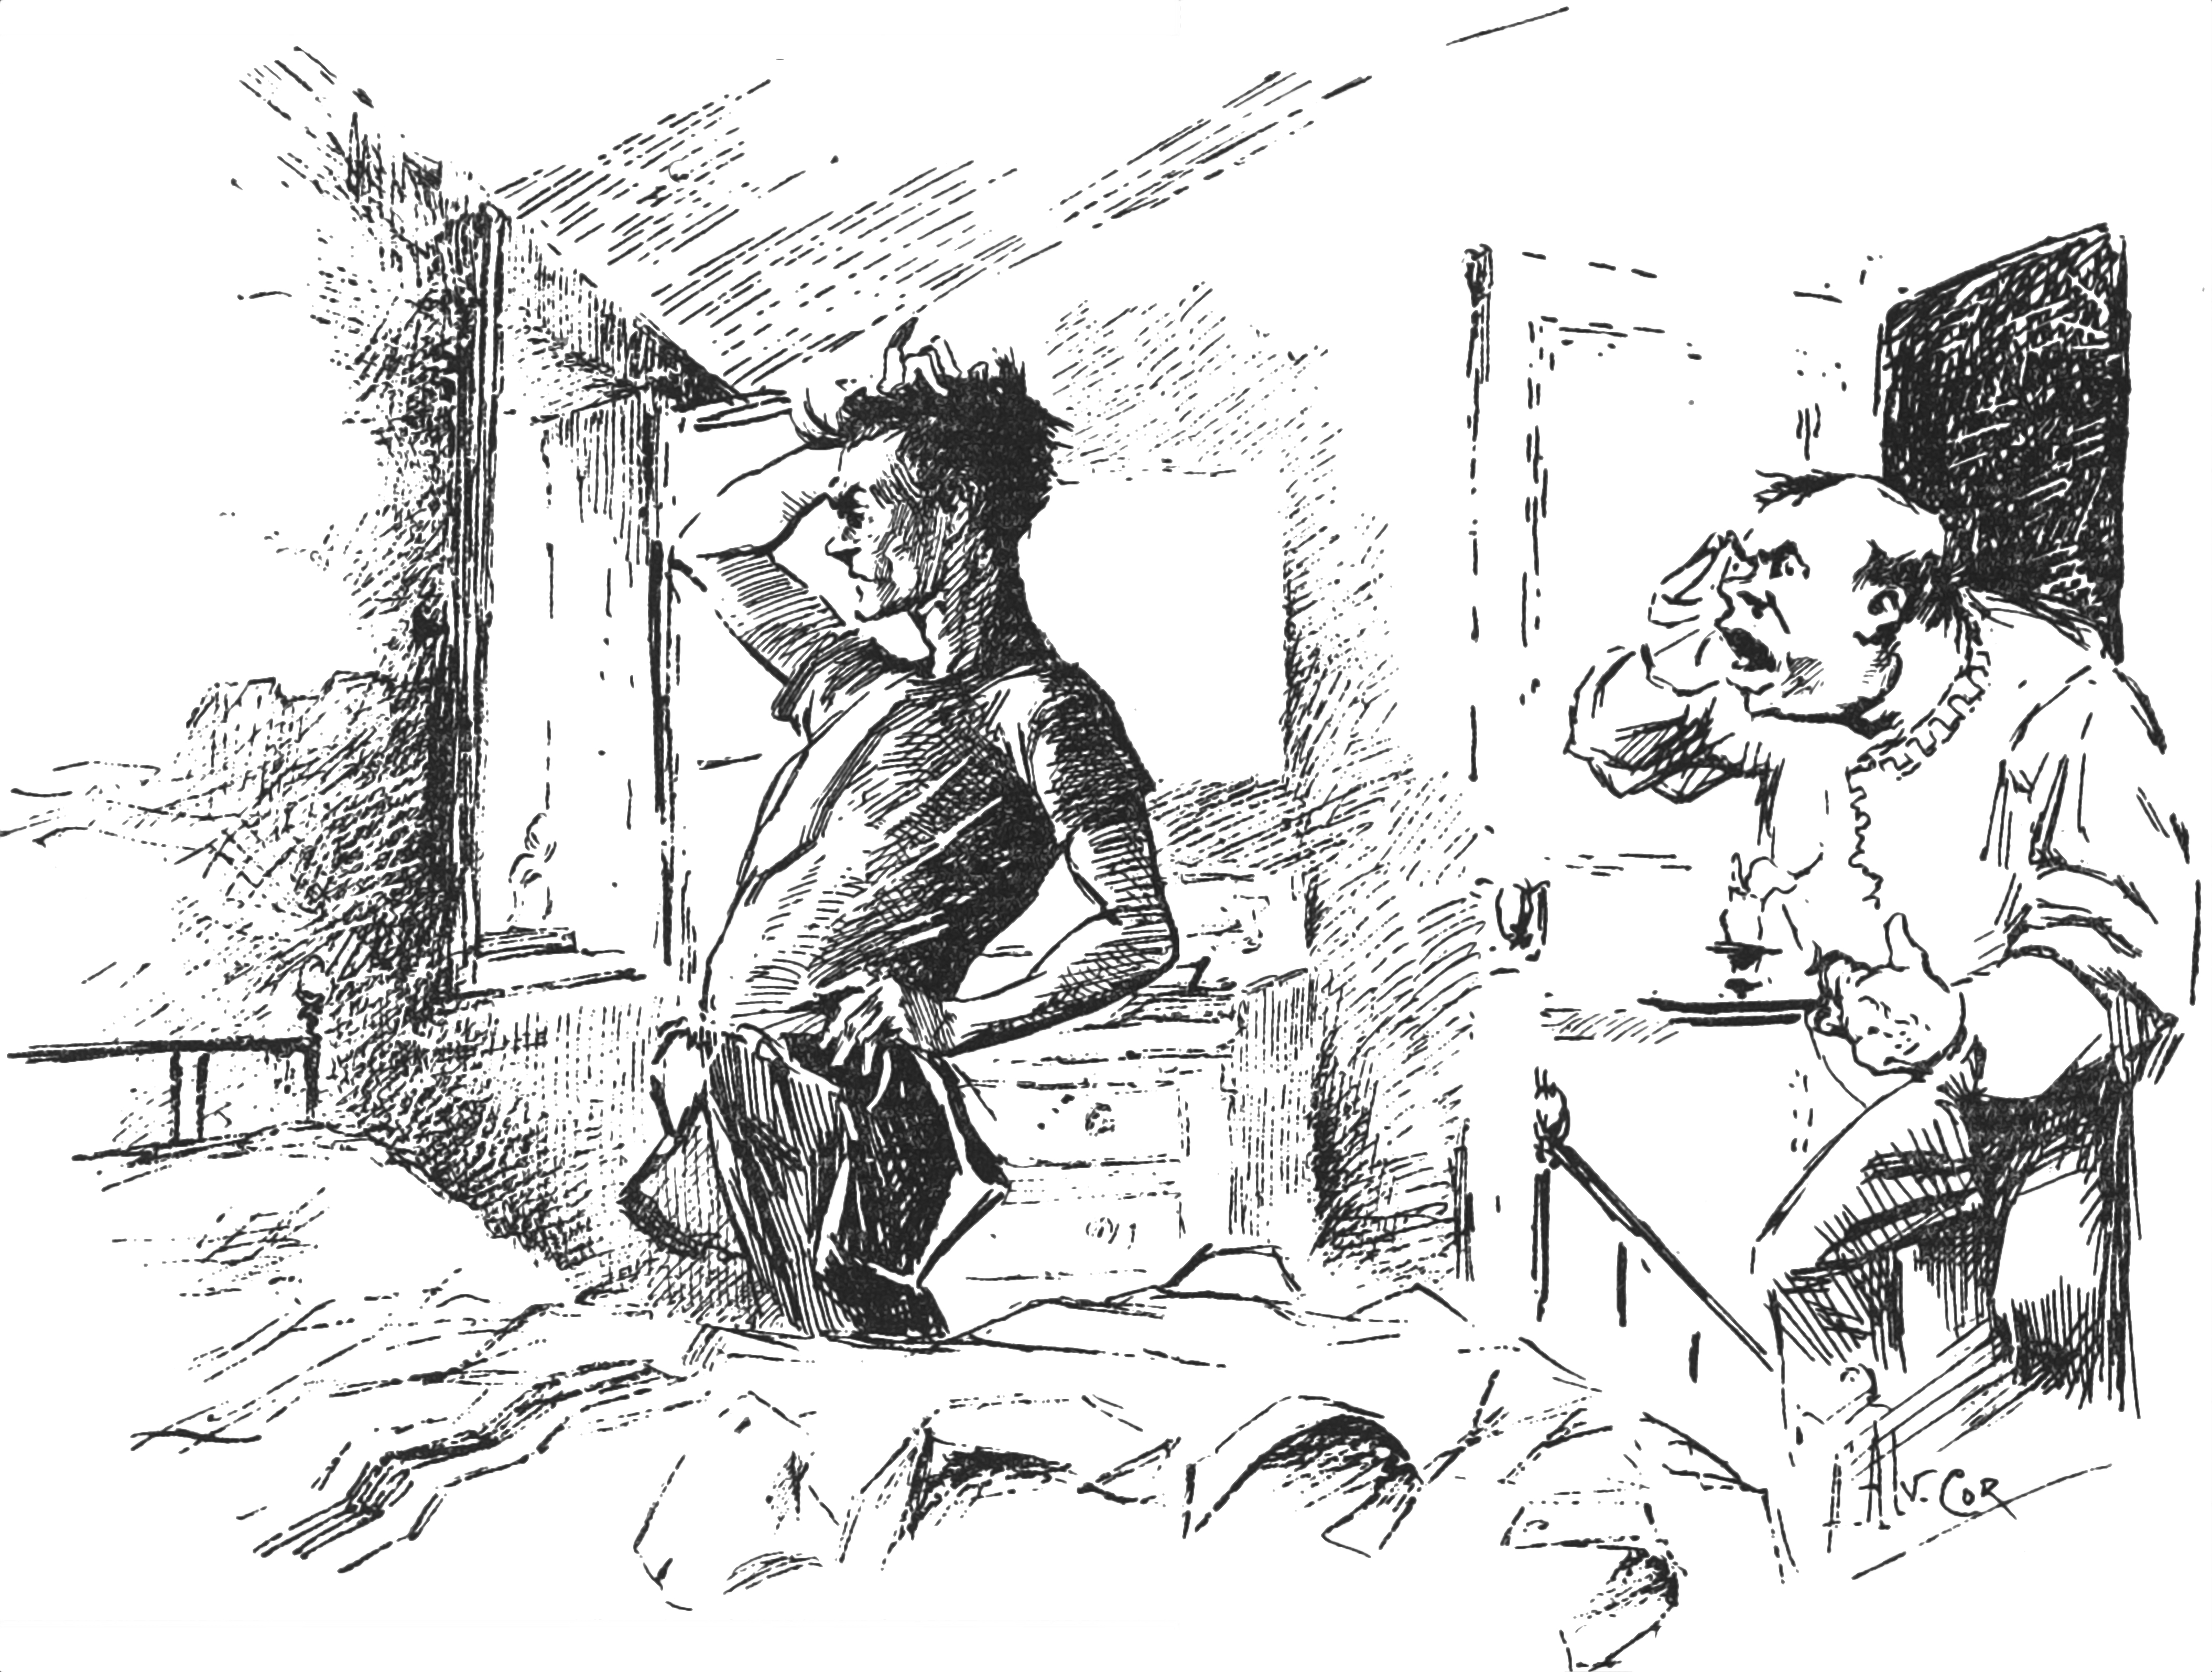
\includegraphics[width=0.5\textwidth]{14bedroom}
%\end{wrapfigure}

\begin{figure}[tb!]
\centering
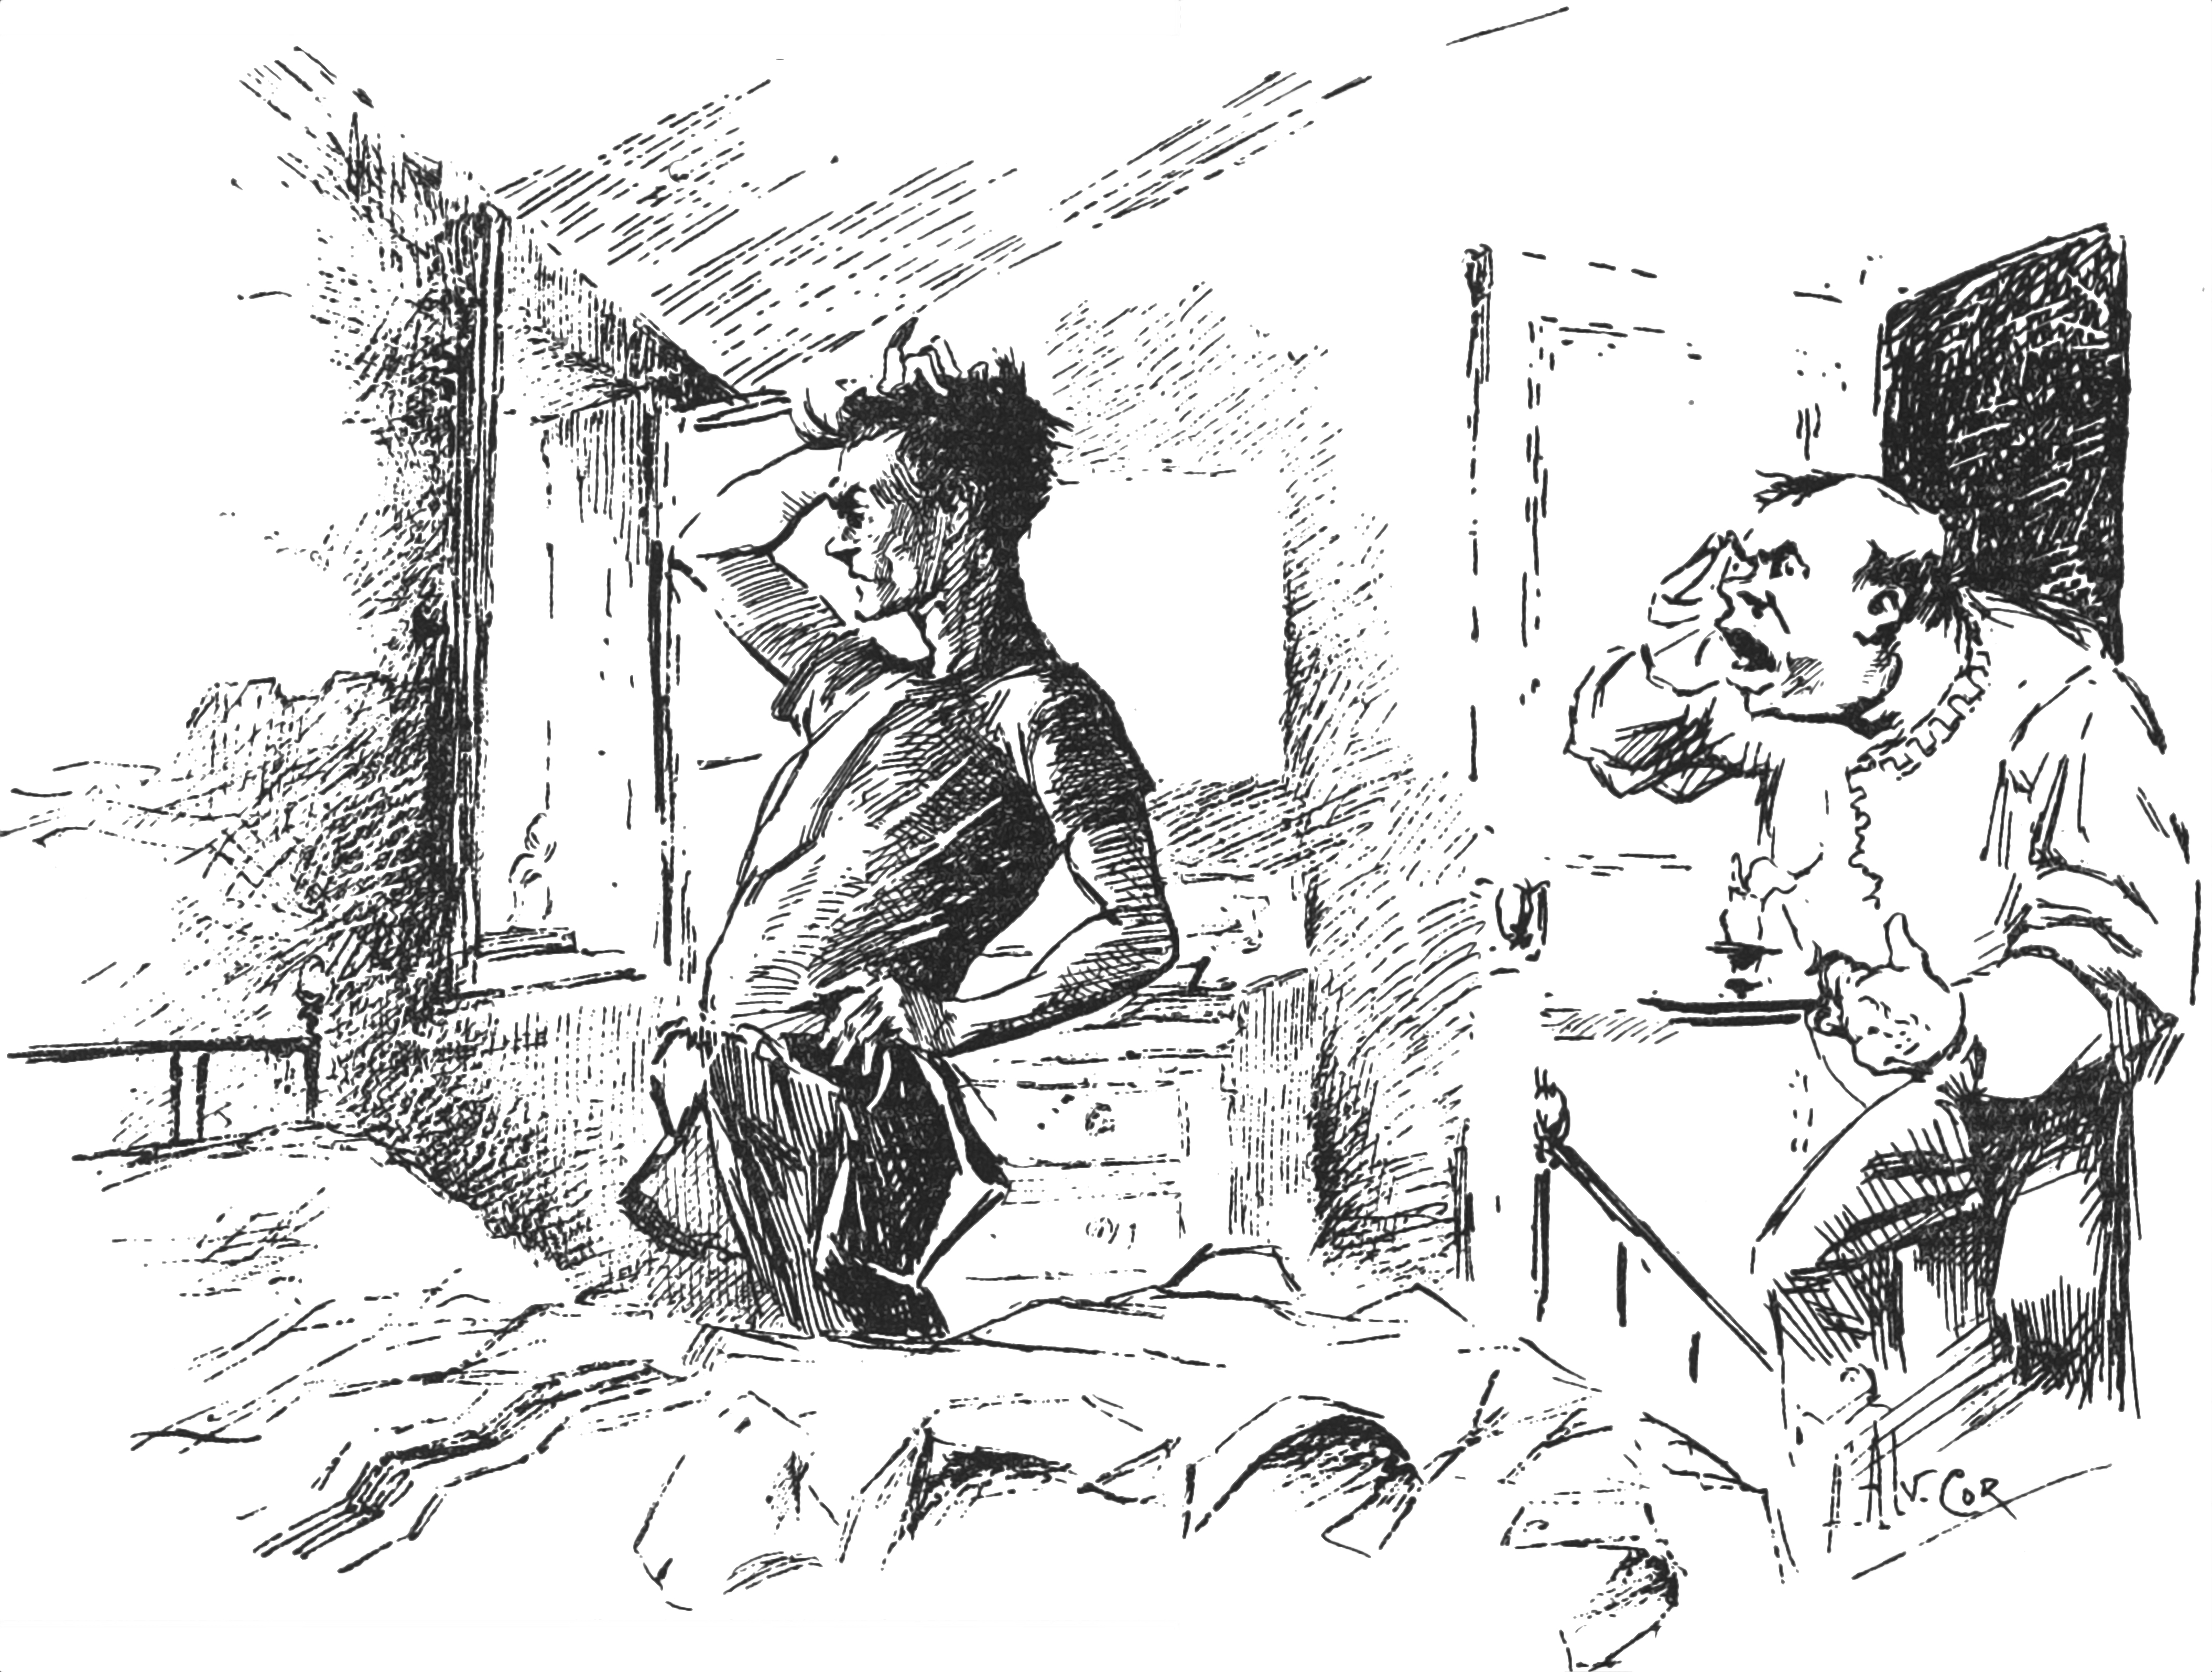
\includegraphics[width=\textwidth]{14bedroom}
\end{figure}

And all about him—in the rooms below, in the houses on each side and across the road, and behind in the Park Terraces and in the hundred other streets of that part of Marylebone, and the Westbourne Park district and St~Pancras, and westward and northward in Kilburn and St~John's Wood and Hampstead, and eastward in Shoreditch and Highbury and Haggerston and Hoxton, and, indeed, through all the vastness of London from Ealing to East Ham—people were rubbing their eyes, and opening windows to stare out and ask aimless questions, dressing hastily as the first breath of the coming storm of Fear blew through the streets. It was the dawn of the great panic. London, which had gone to bed on Sunday night oblivious and inert, was awakened, in the small hours of Monday morning, to a vivid sense of danger.

Unable from his window to learn what was happening, my brother went down and out into the street, just as the sky between the parapets of the houses grew pink with the early dawn. The flying people on foot and in vehicles grew more numerous every moment. »Black Smoke!« he heard people crying, and again »Black Smoke!« The contagion of such a unanimous fear was inevitable. As my brother hesitated on the door-step, he saw another newsvendor approaching, and got a paper forthwith. The man was running away with the rest, and selling his papers for a shilling each as he ran—a grotesque mingling of profit and panic.

And from this paper my brother read that catastrophic dispatch of the Commander-in-Chief:

»The Martians are able to discharge enormous clouds of a black and poisonous vapour by means of rockets. They have smothered our batteries, destroyed Richmond, Kingston, and Wimbledon, and are advancing slowly towards London, destroying everything on the way. It is impossible to stop them. There is no safety from the Black Smoke but in instant flight.«

That was all, but it was enough. The whole population of the great six-million city was stirring, slipping, running; presently it would be pouring \textit{en masse} northward.

»Black Smoke!« the voices cried. »Fire!«

\begin{wrapfigure}{O}{0.5\textwidth}
\centering

\includegraphics[width=0.5\textwidth]{14bell}
\end{wrapfigure}

The bells of the neighbouring church made a jangling tumult, a cart carelessly driven smashed, amid shrieks and curses, against the water trough up the street. Sickly yellow lights went to and fro in the houses, and some of the passing cabs flaunted unextinguished lamps. And overhead the dawn was growing brighter, clear and steady and calm.

He heard footsteps running to and fro in the rooms, and up and down stairs behind him. His landlady came to the door, loosely wrapped in dressing gown and shawl; her husband followed, ejaculating.

As my brother began to realise the import of all these things, he turned hastily to his own room, put all his available money—some ten pounds altogether—into his pockets, and went out again into the streets.

%\begin{figure}[b!]
%\centering
%
\includegraphics[width=.5\textwidth]{14tailpiece}\captionlistentry{Tailpiece to Chapter \thechapter}
%\end{figure}
